\documentclass[hyperref={pdfpagelabels=false}]{beamer}
\usepackage[BoldFont,SlantFont,CJKnumber,CJKchecksingle]{xeCJK}  
\usepackage{lmodern}
\usetheme{CambridgeUS}
%%%%%%%%%%%%%%%%%%%%%%%%%题目,作�
\title{Plankton Classification with Deep Neural Network}  
\author{Jinna Cui} 
\institute{Vision Lab of OUC}
\date{2016.12.25} 
\begin{document}
\logo{
\includegraphics[scale=0.3]{visionouc.jpg}}
\begin{frame}
\titlepage
\end{frame} 
\usepackage{/Users/jinna/Desktop/study/github/Template/styles/zhfontcfg}

\begin{frame}
\frametitle{Table of contents}
\tableofcontents
\end{frame} 


\section{Dataset} 
\begin{frame}
\frametitle{Dataset} 

\textbf{\Large{WHOI-Plankton}}
 \newline
 \newline
\begin{table}[tbp]
\centering  % ???
\begin{tabular}{lccc} 
\hline
Models \ \   &resource &Classes amount &amount \\ \hline  
Training  &Images collected in 2006-2013 &103 &3233806 \\  \hline       
Testing  & Images collected in 2014  &98 &329834 \\  \hline      
\end{tabular}
\caption{\scriptsize{Dataset1}}
\end{table}

\begin{table}[tbp]
\centering  % ???
\begin{tabular}{lccc} 
\hline
Models \ \   &resource &Classes amount &amount \\ \hline  
Training  &Images collected in 2013 &98 &115951 \\  \hline       
Testing  & Images collected in 2014  &98 &63633 \\  \hline      
\end{tabular}
\caption{\scriptsize{Dataset2}}
\end{table}
 \scriptsize{Deleted Classes: mix, Akashiwo, Didinium-sp, kiteflagellates, Leptocylindrus-mediterraneus.}

\end{frame}

\section{Acquire Global Feature} 
\begin{frame}\frametitle{Architecture of Neural Network}
\centering

\begin{figure}[!htb] %插
\centering
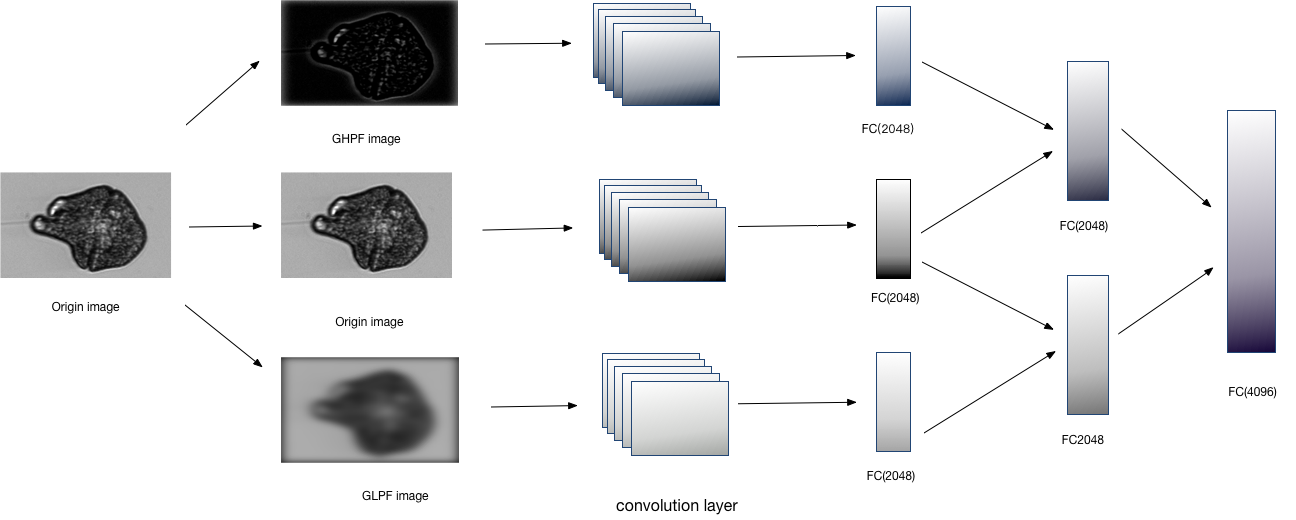
\includegraphics[width=0.8\textwidth]{network}
\end{figure} 
\begin{itemize}

\item 3 channels CNN(share same label)
\end{itemize} 
\end{frame}

\begin{frame}\frametitle{Bilateral Filtering}

\begin{figure}[!ht] 
  \centering 
  \subfigure{ 
    \label{fig:subfig:a} %% label for first subfigure 
    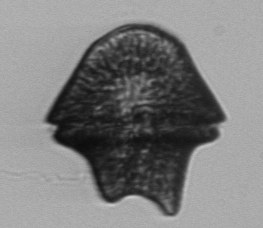
\includegraphics[width=4cm,height=3cm]{1.png}} 
  \hspace{0.01in} 
  \subfigure{ 
    \label{fig:subfig:b} %% label for second subfigure 
    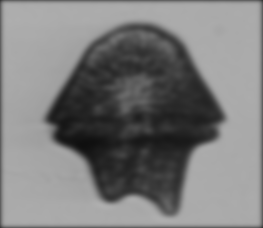
\includegraphics[width=4cm,height=3cm]{5.png}} 
   \hspace{0.02in} 
   \subfigure{ 
    \label{fig:subfig:b} %% label for second subfigure 
    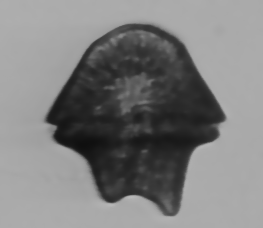
\includegraphics[width=3cm,height=2.5cm]{2.png}} 
   \hspace{0.2in} 
   \subfigure{ 
    \label{fig:subfig:b} %% label for second subfigure 
    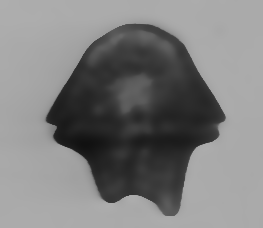
\includegraphics[width=3cm,height=2.5cm]{3.png}} 
   \hspace{0.2in} 
   \subfigure{ 
    \label{fig:subfig:b} %% label for second subfigure 
    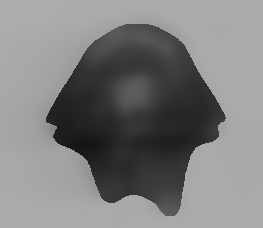
\includegraphics[width=3cm,height=2.5cm]{4.png}} 
   \hspace{0.2in}  
  \label{fig:subfig} %% label for entire figure 
\end{figure}
\end{frame}


\section{Results of My Experiments} 
\begin{frame}\frametitle{Experiments Results}
\centering
\begin{table}[tbp]
\centering  % ???
\begin{tabular}{lccc} 
\hline
Models \ \   &Accuracy\\ \hline  
AlexNet trained on origin images &87.51\% \\  \hline       
AlexNet trained on BF images &81.95\%\\  \hline      
\end{tabular}
\caption{\scriptsize{Experiments Results of Plankton Classification}}
\end{table}
\end{frame}

\section{Database}
\begin{frame}\frametitle{Database}
\centering
\begin{table}[tbp]
\centering  % ???
\begin{tabular}{lcccc} 
\hline
Data \ \   &Total &Mix &Deleted 4 classes &Rest 98 classes \\ \hline  
2013 &394234  &278283 &0 &115951 \\  \hline       
2104 &329834 &266156 &43 &63633\\  \hline      
\end{tabular}
\caption{\scriptsize{Database Analysis}}
\end{table}
????
\end{frame}


\begin{frame}
\center
\huge{Thanks for your attention !}
\end{frame}


\begin{frame}
\center
\Huge{Q \& A}
\end{frame}
\end{document}
